\documentclass[tikz,border=0pt]{standalone}
\usetikzlibrary{shadings,calc}
\definecolor{skytop}{HTML}{060B2A}
\definecolor{skymid}{HTML}{0F1E5A}
\definecolor{skybot}{HTML}{2A3C86}
\definecolor{fw1}{HTML}{FF5E7E}
\definecolor{fw1b}{HTML}{FFC1CF}
\definecolor{fw2}{HTML}{FFD166}
\definecolor{fw2b}{HTML}{FFF3C4}
\definecolor{fw3}{HTML}{6EE7F9}
\definecolor{fw3b}{HTML}{D4FBFF}
\definecolor{lantern}{HTML}{FF8C42}
\definecolor{lanternhi}{HTML}{FFD9A8}
\definecolor{stall}{HTML}{1A1530}
\definecolor{stallroof}{HTML}{C0392B}
\definecolor{stallroof2}{HTML}{F4F1EA}
\definecolor{crowd}{HTML}{05040F}
\definecolor{ground}{HTML}{1C1838}
\definecolor{water}{HTML}{0D1B4B}
\begin{document}
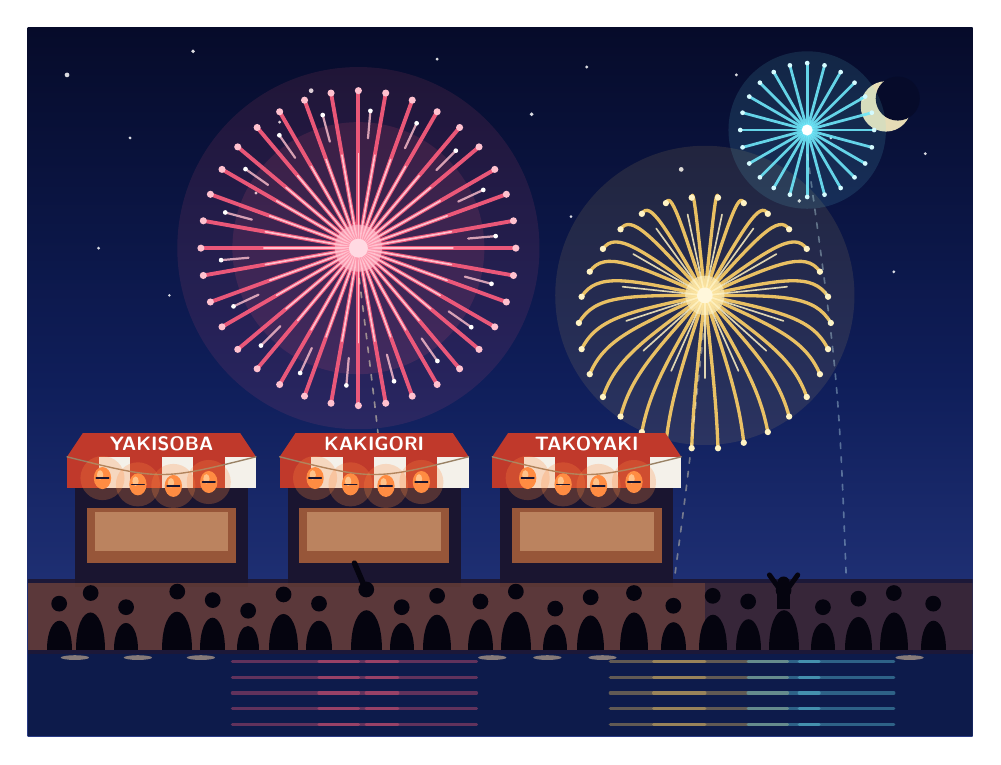
\begin{tikzpicture}[x=1cm,y=1cm,line cap=round,line join=round]
  \clip (0,0) rectangle (12,9);
  % ---- night sky gradient ----
  \shade[top color=skytop,bottom color=skybot,middle color=skymid] (0,0) rectangle (12,9);
  % ---- stars ----
  \foreach \x/\y/\r in {0.5/8.4/0.03,1.3/7.6/0.02,2.1/8.7/0.025,2.9/6.9/0.02,3.6/8.2/0.03,5.2/8.6/0.02,6.4/7.9/0.025,7.1/8.5/0.02,8.3/7.2/0.03,9.0/8.4/0.02,9.8/6.8/0.025,10.6/8.1/0.03,11.4/7.4/0.02,0.9/6.2/0.02,11.0/5.9/0.02,4.4/6.4/0.02,1.8/5.6/0.018,10.2/7.6/0.02,6.9/6.6/0.018,3.2/7.8/0.02}{
    \fill[white,opacity=0.85] (\x,\y) circle (\r);
  }
  % ---- crescent moon ----
  \fill[fw2b,opacity=0.9] (10.9,8.0) circle (0.32);
  \fill[skytop] (11.05,8.1) circle (0.28);

  % ---- firework 1: big pink chrysanthemum (centre-left) ----
  \begin{scope}[shift={(4.2,6.2)}]
    \fill[fw1,opacity=0.10] (0,0) circle (2.3);
    \fill[fw1,opacity=0.12] (0,0) circle (1.6);
    \foreach \a in {0,10,...,350}{
      \draw[fw1,line width=1.4pt,opacity=0.9] (0,0) -- (\a:2.0);
      \draw[fw1b,line width=0.6pt] (0,0) -- (\a:1.2);
      \fill[fw1b] (\a:2.0) circle (0.045);
    }
    \foreach \a in {5,25,...,355}{
      \draw[fw1b,line width=0.8pt,opacity=0.8] (\a:1.4) -- (\a:1.75);
      \fill[white] (\a:1.75) circle (0.03);
    }
    \fill[white] (0,0) circle (0.12);
    \fill[fw1b,opacity=0.6] (0,0) circle (0.3);
  \end{scope}

  % ---- firework 2: golden willow (right) ----
  \begin{scope}[shift={(8.6,5.6)}]
    \fill[fw2,opacity=0.10] (0,0) circle (1.9);
    \foreach \a in {0,12,...,348}{
      \draw[fw2,line width=1.2pt,opacity=0.9] (0,0) .. controls (\a:1.0) and (\a:1.4) .. ($(\a:1.6)+(0,-0.35)$);
      \fill[fw2b] ($(\a:1.6)+(0,-0.35)$) circle (0.04);
    }
    \foreach \a in {6,30,...,354}{
      \draw[fw2b,line width=0.6pt,opacity=0.85] (0,0) -- (\a:1.05);
    }
    \fill[white] (0,0) circle (0.1);
    \fill[fw2b,opacity=0.6] (0,0) circle (0.25);
  \end{scope}

  % ---- firework 3: small cyan burst (upper right, further away) ----
  \begin{scope}[shift={(9.9,7.7)}]
    \fill[fw3,opacity=0.12] (0,0) circle (1.0);
    \foreach \a in {0,15,...,345}{
      \draw[fw3,line width=1pt,opacity=0.9] (0,0) -- (\a:0.85);
      \fill[fw3b] (\a:0.85) circle (0.03);
    }
    \fill[white] (0,0) circle (0.07);
  \end{scope}
  % rising trails
  \draw[fw2b,line width=0.6pt,opacity=0.5,dash pattern=on 2pt off 3pt] (4.6,1.9) .. controls (4.5,3.5) .. (4.2,5.9);
  \draw[fw2b,line width=0.6pt,opacity=0.4,dash pattern=on 2pt off 3pt] (8.2,1.9) .. controls (8.4,3.4) .. (8.6,5.3);
  \draw[fw3b,line width=0.6pt,opacity=0.35,dash pattern=on 2pt off 3pt] (10.4,1.9) .. controls (10.3,4.5) .. (9.9,7.4);

  % ---- river with reflections (bottom band) ----
  \fill[water] (0,0) rectangle (12,1.1);
  \foreach \x/\c/\w in {3.4/fw1/1.6,4.2/fw1/1.0,5.0/fw1/1.4,8.0/fw2/1.2,8.8/fw2/1.7,9.6/fw3/0.9,10.4/fw3/1.2}{
    \foreach \y in {0.15,0.35,0.55,0.75,0.95}{
      \draw[\c,opacity=0.35,line width=1.2pt] (\x-\w/2,\y) -- (\x+\w/2,\y);
    }
  }
  % ---- riverbank ground ----
  \fill[ground] (0,1.05) rectangle (12,2.0);

  % ---- food stalls with lanterns ----
  \foreach \sx in {0.6,3.3,6.0}{
    \begin{scope}[shift={(\sx,1.9)}]
      % stall body
      \fill[stall] (0,0) rectangle (2.2,1.25);
      % counter glow
      \fill[lantern,opacity=0.55] (0.15,0.3) rectangle (2.05,1.0);
      \fill[lanternhi,opacity=0.35] (0.25,0.45) rectangle (1.95,0.95);
      % striped awning
      \foreach \i in {0,...,5}{
        \pgfmathparse{int(mod(\i,2))}
        \ifnum\pgfmathresult=0 \fill[stallroof] (\i*0.4-0.1,1.25) rectangle (\i*0.4+0.3,1.65);
        \else \fill[stallroof2] (\i*0.4-0.1,1.25) rectangle (\i*0.4+0.3,1.65); \fi
      }
      \fill[stallroof] (-0.1,1.65) -- (2.3,1.65) -- (2.1,1.95) -- (0.1,1.95) -- cycle;
      % lantern string
      \draw[lanternhi!60!black,line width=0.5pt] (-0.1,1.65) .. controls (1.1,1.35) .. (2.3,1.65);
      \foreach \lx/\ly in {0.35/1.5,0.8/1.42,1.25/1.4,1.7/1.45}{
        \fill[lantern,opacity=0.25] (\lx,\ly-0.12) circle (0.28);
        \fill[lantern] (\lx,\ly-0.12) ellipse (0.11 and 0.14);
        \fill[lanternhi,opacity=0.7] (\lx-0.03,\ly-0.08) ellipse (0.04 and 0.06);
        \draw[stall,line width=0.5pt] (\lx-0.08,\ly-0.12) -- (\lx+0.08,\ly-0.12);
      }
    \end{scope}
  }
  % stall signs
  \node[font=\sffamily\bfseries\scriptsize,text=white] at (1.7,3.72) {YAKISOBA};
  \node[font=\sffamily\bfseries\scriptsize,text=white] at (4.4,3.72) {KAKIGORI};
  \node[font=\sffamily\bfseries\scriptsize,text=white] at (7.1,3.72) {TAKOYAKI};

  % warm lantern light falling on the bank (behind the crowd)
  \fill[lantern,opacity=0.28] (0,1.1) rectangle (8.6,1.95);
  \fill[lantern,opacity=0.12] (8.6,1.1) rectangle (12,1.95);
  % ---- crowd silhouettes along the riverbank ----
  \foreach \px/\ph/\pw in {0.4/0.55/0.16,0.8/0.7/0.18,1.25/0.5/0.15,1.9/0.72/0.19,2.35/0.6/0.16,2.8/0.45/0.14,3.25/0.68/0.18,3.7/0.55/0.16,4.3/0.75/0.2,4.75/0.5/0.15,5.2/0.66/0.18,5.75/0.58/0.16,6.2/0.72/0.19,6.7/0.48/0.15,7.15/0.64/0.17,7.7/0.7/0.18,8.2/0.52/0.16,8.7/0.66/0.18,9.15/0.58/0.16,9.6/0.74/0.19,10.1/0.5/0.15,10.55/0.62/0.17,11.0/0.7/0.18,11.5/0.55/0.16}{
    % body
    \fill[crowd] (\px-\pw,1.1) .. controls (\px-\pw,1.1+\ph*0.9) and (\px+\pw,1.1+\ph*0.9) .. (\px+\pw,1.1) -- cycle;
    % head
    \fill[crowd] (\px,1.1+\ph*0.9+0.09) circle (0.1);
  }
  % a few raised arms / child on shoulders
  \draw[crowd,line width=2pt] (4.3,1.85) -- (4.15,2.2);
  \fill[crowd] (9.6,1.95) circle (0.08) (9.6,1.75) rectangle (9.6,1.75);
  \fill[crowd] (9.52,1.62) rectangle (9.68,1.88);
  \draw[crowd,line width=1.8pt] (9.6,1.8) -- (9.42,2.05) (9.6,1.8) -- (9.78,2.05);


  % ---- sparkler glints on the water surface near the bank ----
  \foreach \x in {0.6,1.4,2.2,5.9,6.6,7.3,11.2}{\fill[lanternhi,opacity=0.5] (\x,1.0) ellipse (0.18 and 0.03);}
\end{tikzpicture}
\end{document}
